% Results: Use your models to draw some conclusions.
    % Were all three binary classification problems equally predictible?
    % Were all the tested models equally “good”?
    % Did dimension reduction have a meaningful (negative or positive) impact?
    % Given the motivation, what would you recommend?
    % Include at least one figure to support your conclusions.

\graphicspath{ {../images/} }

\subsection{Model performance on standardized data}

The metric we choose is Accuracy, which is commonly used as an evaluation metric for prediction problems, including predicting customer income levels based on consumer personality analysis datasets for different marital statuses. However, the suitability of using accuracy as the primary metric depends on the specific characteristics of the problem and the dataset. Here are some reasons why accuracy might be a reasonable choice for this particular problem:

Balanced class distribution: If the classes (income levels) in the dataset are relatively balanced across different marital statuses, accuracy can provide a good overall measure of the model's performance. When classes are imbalanced, accuracy may not be the best metric as it can be skewed towards the majority class.

Equal misclassification costs: Accuracy assumes that the cost of misclassifying an instance into any other class is equal. In the context of customer income level prediction, this assumption might be reasonable if the consequences of misclassifying a customer into a higher or lower income level are similar.

Interpretability: Accuracy is a straightforward and interpretable metric. It represents the proportion of correctly classified instances, which can be easily understood by stakeholders and decision-makers.

Baseline comparison: Accuracy provides a baseline for comparing the performance of different models or algorithms. If the goal is to achieve the highest possible accuracy, it serves as a useful metric for model selection and optimization.

K-fold cross-validation provides a more accurate and reliable estimate of a model's performance on unseen data compared to using a single train-test split. By training and evaluating the model on multiple folds, the performance estimate is less prone to bias or variance due to the specific way the data was partitioned.

To get a reliable result for binary classification, we use 5-fold validation for tuning the hyperparameters of our models. The hyperparameters are recorded under each experimentation. Some results with large variance are not recorded and requires more investigation.

\begin{figure}[h]
    \centering
    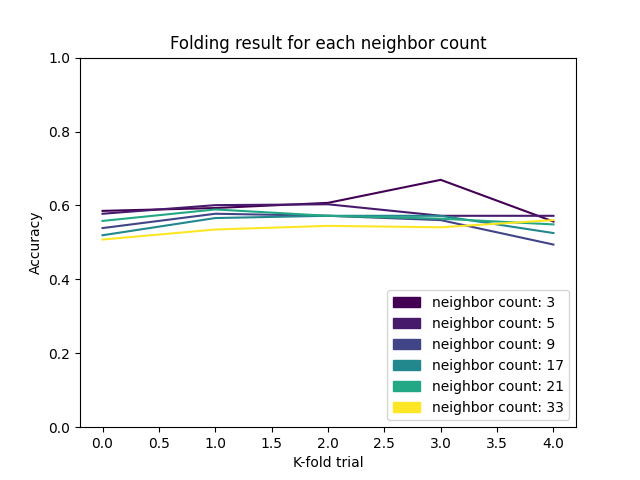
\includegraphics[width=\textwidth]{images/folding_count.png}
    \caption{5-fold visualization for different hyperparameters in KNN}
    \label{feature_fit}
    \end{figure}

The result for 5-fold and prediction accuracy are as follows:

\begin{table}[h!]
    \centering
\begin{tabular}{ |p{3cm}||p{5cm}|p{4cm}|p{4cm}|}
    \hline
    \multicolumn{4}{|c|}{Model performance for income level from sigle population (non-reduced)} \\
    \hline
    Model Name& Training time (seconds)& Training precision & Testing precision \\
    \hline
    SVM &0.0110    &0.92&0.91\\
    ANN &2.94  & 0.93  & 0.92\\
    KNN &0.0000 & 0.90&0.89\\
    RFC &0.1406 & 0.93&0.91\\
    \hline
   \end{tabular}
\end{table}

In this population, the (potentially) best hyperparameters for income level from sigle population (non-reduced) are as follows:

SVM best: $C =1, kernel = linear$
For the SVM model:
C = 1: The parameter C is a regularization parameter that helps control the trade-off between achieving a low error on the training data and minimizing the model complexity for better generalization. A C value of 1 provides a good balance, preventing the model from fitting the training data too closely (overfitting).
Kernel = Linear: The linear kernel is simple and effective for linearly separable data. Using a linear kernel often requires less computation and avoids the risk of overfitting when the data is not complex.

ANN best: $unit = 5, activation = relu, lr = 0.01, batch\_size = 16$.

For the ANN model:
Units = 5: This refers to the number of neurons in the hidden layer. Having 5 units is a choice that can capture sufficient complexity in the data without overcomplicating the model, which can help in avoiding overfitting and reducing computational demand.
Activation = ReLU (Rectified Linear Unit): ReLU is a popular activation function because it introduces non-linearity into the model without affecting the gradients too much, which helps in avoiding the vanishing gradient problem common with other activation functions like sigmoid or tanh.
Learning Rate = 0.01: This is a moderate learning rate that helps ensure the model learns at a reasonable pace; not too fast to skip optimal solutions, and not too slow to impede the learning process.
Batch Size = 16: This batch size is small enough to allow the model to update its weights frequently, which can lead to faster convergence. Small batches can also provide a regularizing effect and lower the risk of overfitting.

\begin{table}[h!]
    \centering
    \begin{tabular}{ |p{3cm}||p{5cm}|p{4cm}|p{4cm}|}
    \hline
    \multicolumn{4}{|c|}{Model performance for income level from no long time relationships population (non-reduced)}\\
    \hline
    Model Name& Training time (seconds)& Training precision & Testing precision \\
    \hline
    SVM &0.0020   &0.84&0.92\\
    ANN &0.24  & 0.94 & 0.91\\
    KNN &0.0000 & 0.88&0.86\\
    RFC & 0.4865 & 0.90&0.8\\
    \hline
   \end{tabular}
\end{table}

The (potentially) best hyperparameters for income level from no long time relationships population (non-reduced) are:

SVM:
Best parameters: $\{'C': 100, 'kernel': 'rbf'\}$

ANN:
Best hyperparameters: $\{'units': 5, 'activation': 'relu', 'learning_rate': 0.1, 'epochs': 20, 'batch\_size': 16, 'accuracy': 0.9125909752547308, 'time': 2.878108024597168\}$

KNN:
Best parameters: $\{'n_neighbors': 33\}$

RFC:
Best parameters: $\{'max_samples': 0.7, 'n_estimators': 256\}$

\begin{table}[h!]
    \centering
    \begin{tabular}{ |p{3cm}||p{5cm}|p{4cm}|p{4cm}|}
    \hline
    \multicolumn{4}{|c|}{Model performance for income level from married population (non-reduced)} 
     \\
    \hline
    Model Name& Training time (seconds)& Training precision & Testing precision \\
    \hline
    SVM &0.0020   &0.87&0.92\\
    ANN &0.95  & 0.92 & 0.92\\
    KNN &0.0000 & 0.90&0.91\\
    RFC &0.3014 & 0.91&0.92\\
    \hline
   \end{tabular}
\end{table}

The (potentially) best hyperparameters for income level from married population (non-reduced) are:

SVM:
Best parameters: $\{'C': 100, 'kernel': 'rbf'\}$

ANN:
Best hyperparameters: $\{'units': 5, 'activation': 'relu', 'learning\_rate': 0.1, 'epochs': 20, 'batch\_size': 16, 'accuracy': 0.9125909752547308, 'time': 2.878108024597168\}$

KNN:
Best parameters: $\{'n\_neighbors': 33\}$

RFC:
Best parameters: $\{'max\_samples': 0.7, 'n\_estimators': 256\}$

\subsection{Dimension reducing techniques}
After reducing the variables, most models gets worse performance. The model performance are as follows:

\begin{table}[h!]
    \centering
\begin{tabular}{ |p{3cm}||p{5cm}|p{4cm}|p{4cm}|}
    \hline
    \multicolumn{4}{|c|}{Model performance for income level from single population (reduced)} \\
    \hline
    Model Name& Training time (seconds)& Training precision & Testing precision \\
    \hline
    SVM &0.0110    &0.91&0.89\\
    ANN &2.9526  & 0.893  & 0.90\\
    KNN &0.0000 & 0.86&0.83\\
    RFC &0.0427 & 0.89&0.91\\
    \hline
   \end{tabular}
\end{table}

The (potentially) best hyperparameters for income level from single population (reduced) are:

ANN:
Best hyperparameters: $\{'units': 10, 'activation': 'tanh', 'learning\_rate': 0.01, 'epochs': 20, 'batch\_size': 16\}$

SVM:
Best hyperparameters: $\{'C': 10, 'kernel': 'poly'\}$

KNN:
Best parameters: $\{'n\_neighbors': 3\}$

RFC:
Best parameters: $\{'max\_samples': 0.9, 'n\_estimators': 16\}$

\begin{table}[h!]
    \centering
    \begin{tabular}{ |p{3cm}||p{5cm}|p{4cm}|p{4cm}|}
    \hline
    \multicolumn{4}{|c|}{Model performance for income level from no long time relationships population (reduced)}\\
    \hline
    Model Name& Training time (seconds)& Training precision & Testing precision \\
    \hline
    SVM &0.0020   &0.83&0.89\\
    ANN &0.6231  & 0.86 & 0.82\\
    KNN &0.0000 & 0.84&0.83\\
    RFC & 0.469 & 0.88&0.86\\
    \hline
   \end{tabular}
\end{table}

The (potentially) best hyperparameters for income level from married population (reduced) are:

KNN:
Best parameters: $\{'n\_neighbors': 33\}$

RFC:
Best parameters: $\{'max\_samples': 0.5, 'n\_estimators': 16\}$

\begin{table}[h!]
    \centering
    \begin{tabular}{ |p{3cm}||p{5cm}|p{4cm}|p{4cm}|}
    \hline
    \multicolumn{4}{|c|}{Model performance for income level from married population (reduced)} 
     \\
    \hline
    Model Name& Training time (seconds)& Training precision & Testing precision \\
    \hline
    SVM &0.007   &0.89&0.9\\
    ANN &0.9544  & 0.892 & 0.86\\
    KNN &0.0000 & 0.87&0.9\\
    RFC &1.0349 & 0.91&0.92\\
    \hline
   \end{tabular}
\end{table}

The (potentially) best hyperparameters for income level from married population (reduced) are:

KNN:
Best parameters: $\{'n\_neighbors': 33\}$

RFC:
Best parameters: $\{'max\_samples': 0.9, 'n\_estimators': 512\}$

As the analysis show, it is practical to predict a person's income level with those given data. The companies could use such a model to segment their target audience more effectively based on predicted income levels. They could tailor their marketing campaigns, messaging, and advertising content to resonate better with different income groups, increasing the likelihood of successful conversions and sales.

In E-commerce and retail businesses. With sufficient data, we can predict customers' income levels, these businesses could personalize product recommendations, promotions, and user experiences accordingly.

They could offer more relevant products, services, or content to different customer segments, improving customer satisfaction and potentially increasing sales.


